                                                                                                                                                                                                                                                                                                                                                                                                                                                                                                               
\chapter{Numerical Computation of Motion about the Lagrange Points}

\lettrine{T}{he} construction of low-energy transfers requires the implementation of numerical techniques and methods. The following section introduces and discusses key methods and tools to analyse and construct low-energy transfers in the three-body problem. These methods are then demonstrated in the construction of a Halo orbit using single forward shooting techniques.

PERHAPS AN INTRODUCTION TO THE NUMERICAL COMPUTATION WORK SO FAR???

\section{Poincayrei maps}

\section{The State Transition Matrix}

The state transition matrix is a key tool for monitoring divergent dynamics through a trajectory. For the purposes of the construction of orbital transfers, it has the following uses:

\begin{itemize}
\item  providing a means of adjusting initial conditions of a trajectory to correct for variations in desired final conditions;
\item providing a means of examination of orbit stability, and eigenvector orientations \citep{Parker2014}.
\end{itemize}

 To this end, the state transition matrix is essential for differential correction techniques (Section \ref{s:differentialcorrection}). As in \citep{Howell1997}, if we suppose that we have some state vector at a time $t$, $\pmb{\bar{x}} = [ x, y, z, \dot{x}, \dot{y}, \dot{z} \big ]^T$, we may obtain an approximation relative to some reference solution using a Taylor series expansion. Ignoring higher order terms, this computes as:
 
 \begin{equation}\label{eq:taylorseriesstatematrix}
 \delta \pmb{\dot{x}} = A\left(t\right) \delta \pmb{\bar x} \left(t\right)
 \end{equation}

where $A\left(t\right)$ is a 6x6 time varying matrix of 3x3 sub-matrices:

\begin{equation}\label{eq:jacobianequation}
A\left(t\right) = 
\begin{bmatrix}
0 & I_3 \\
U & 2~\Omega
\end{bmatrix}
\end{equation}
with

\begin{equation}
\Omega = 
\begin{bmatrix}
0 & 1 & 0 \\
-1 & 0 & 0 \\
0 & 0 & 0
\end{bmatrix}
\end{equation}

and

\begin{equation}
U = 
\begin{bmatrix}
U_{xx} & U_{xy} & U_{xz} \\
U_{yx} & U_{yy} & U_{yz} \\
U_{zx} & U_{zy} & U_{zz}
\end{bmatrix}
\end{equation}

where $U_{ab}$ represents $\frac{\partial U}{\partial a~\partial b}$, and $U$ is symmetric if all derivatives of all orders are continuous. Referring back to Equation \ref{eq:taylorseriesstatematrix}, we note the solution of Equation \ref{eq:taylorseriesstatematrix} is of the form:

\begin{equation}
\delta \pmb{\dot{x}} \left( t \right) = \Phi \left(t, t_0 \right) \delta \pmb{x} \left(t_0\right)
\end{equation}

where $\Phi \left(t, t_0 \right)$ implies the state transition matrix propagated from time $t_0$ to time $t$. The elements of $\Phi$ correspond to the matrix partial, which represents the sensitivity in the state at time $t$ following a small perturbation at time $t_0$.

\begin{equation}\label{eq:statematrixpartial}
\Phi \left( t \right) = \frac{\partial \pmb{x} \left( t \right)}{\partial \pmb{x} \left( t_0 \right)}
\end{equation}

\noindent Differentiation of Equation \ref{eq:statematrixpartial} and substitution of Equations \ref{eq:taylorseriesstatematrix} and \ref{eq:statematrixpartial} yields:

\begin{equation}
\delta \pmb{\dot{x}} = A \left( t \right) \delta \pmb{x} \left( t \right) = \dot{\Phi}\left(t, t_0\right) \delta \pmb{x} \left( t_0 \right) + \Phi \left(t, t_0\right) \delta\pmb{\dot{x}}\left(t_0\right) = A \left( t \right) \delta \pmb{x} \left( t \right) = \dot{\Phi}\left(t, t_0\right) \delta \pmb{x} \left( t_0 \right)
\end{equation}

\noindent and thus

\begin{equation}\label{eq:finishedstatematrixeq}
\dot{\Phi} \left( t, t_0 \right) = A\left( t\right)\Phi(t, t_0)
\end{equation}

\noindent which represents 36 first order differential equations for iteration through the orbit propagation\footnote{These equations are also known as the variational equations}. The initial conditions for Equation \ref{eq:finishedstatematrixeq} are provided by a $6\times 6$ identity matrix.

\subsection{The Monodromy Matrix and Floquet's Theorem}

A special case of the state transition matrix, the monodromy matrix provides a determination of the stability of a periodic orbit \citep{Russell2006}; for an unstable orbit, the monodromy matrix yields at least one eigenvalue outside the unit circle. In the CR3BP, the monodromy matrix typically contains 6 eigenvalues occurring in reciprocal pairs \citep{broucke1968}, $\lambda_i$, $i = 1, 2, ..., 6$, corresponding to six eigenvectors $\pmb{v}_i$. These eigenvalues are roots of a characteristic equation, with a characteristic exponent $e^{\alpha T}$, where $T$ is the period of the orbit\footnote{This exponent is sometimes referred to as the Lyapunov characteristic exponent.}. The computation of the eigenvalue reveals the stability of the periodic orbit under a perturbation; referring to Table \ref{table:eigenvalues}:

\begin{itemize}
\item We say an orbit is stable if the eigenvalues are in the range (-1, 1);
\item an orbit is neutrally stable if the eigenvalue is equal to -1 or 1;
\item an orbit is unstable if the eigenvalue is outside the range [-1, 1];
\end{itemize}

\noindent \citep{broucke1968} states that it is customary to ignore the invariant presence of unity eigenvalues when assessing stability. Broucke also provides a computationally fast method for the determination of eigenvalues $\lambda_1$ through $\lambda_6$:

\begin{table*}[h]\label{tbl:lyapunovexponent}
\centering
\begin{tabular}{l r}
\toprule
\toprule
\textbf{Eigenvalue} & \textbf{Result of Perturbation} \\ \toprule
Real, $< 1$, $> -1$ & Exponential decay \\
Real, $=1$ or $=-1$ & Neither decay nor growth\\
Real, $\geq 1$, $\leq 1$ & Exponential growth\\
Imaginary & The perturbation oscillates about the spacecraft's original state \\
\bottomrule
\bottomrule
\end{tabular}
\caption{Effects of Lyapunov characteristic exponent on perturbation state for a periodic orbit}
\end{table*}

\begin{equation}
\textnormal{det}\left(M - \lambda I\right) = \\ (\lambda - \lambda_1)(\lambda - \lambda_2)(\lambda - \lambda_3)(\lambda - \lambda_4)(\lambda - \lambda_5)(\lambda - \lambda_6) = 0 = (\lambda - 1)^2 ( \lambda - \lambda_1)(\lambda-1/\lambda_1)(\lambda-\lambda_3)(\lambda - 1/\lambda_3)
\end{equation}

\noindent which, if written in terms of intermediate variables $p$ and $q$:

\begin{equation}\label{eq:pandqequation}
(\lambda - 1)^2 = 0;~\lambda^2 + p\lambda + 1 = 0;~\lambda^2 + q\lambda + 1 = 0
\end{equation}

\noindent with $p = -(\lambda_1 + 1/\lambda_1)$, $q = (-\lambda_3 + 1/\lambda_3)$. Factoring \ref{eq:pandqequation} yields:

\begin{equation}\label{eq:factoredpandq}
(\lambda-1)^2\lambda^4 + (p+q)\lambda^3 + (pq+2)\lambda^2 + (p+q)\lambda + 1 = 0
\end{equation}

\noindent and with the introduction of another set of new parameters $\beta$, $\gamma$ and $\delta$, we observe:

\begin{equation}
(\lambda-1)^2\lambda^4 + \beta \lambda^3 + \gamma \lambda^2 + \beta \lambda + \delta = 0
\end{equation}

\noindent which implies $\beta = p+q$, $\gamma = pq + 2$ and $\delta = 1$. Working backwards from these parameters can yield values of the eigenvalues:

\begin{align}
\beta = 2 - \textnormal{trace}(M) \\
\gamma = \frac{\beta^2 - \textnormal{trace}(M^2)}{2} + 1
\end{align}

\noindent then

\begin{equation}
p,~q = \frac{\beta \pm \sqrt{\beta^2 - 4\gamma+8}}{2}
\end{equation}

\noindent and

\begin{equation}
\lambda_1,~1/\lambda_1 = \frac{-p \pm \sqrt{p^2 - 4}}{2}
\end{equation}
\begin{equation}
\lambda_3,~1/\lambda_3 = \frac{-q \pm \sqrt{q^2 - 4}}{2}
\end{equation}

\noindent Combining this with the invariant-unity eigenvalue pair yields the six eigenvalues of the monodromy matrix in the CR3BP, the eigenvectors for which can be computed through use of $M\pmb{v}^2_i = \lambda_i\pmb{v}_i$. If they exist, the stable and unstable eigenvalues are given by the smallest and largest real eigenvalues, respectively.

\section{Differential Correction}\label{s:differentialcorrection}

\subsection{Single-shooting}\label{s:singleshooting}

\section{Construction of a Periodic Orbit using Differential Correction}

We wish to demonstrate the techniques outlined in the previous section by computing a periodic orbit around a Lagrangian point $L_i$, and use this result to introduce the concept of stable and unstable manifolds. Section \ref{s:constructiontheory} outlines the mathematical relations behind the construction of such an orbit, and Section \ref{s:appliedconstruction} provides information on its' implementation in a numerical computation package.

\subsection{Establishing the differential correction routines}

As mentioned in Section \ref{s:singleshooting}, the construction of a full periodic orbit around one of the Lagrangian points requires first the generation of a smaller `seed' orbit to power the differential correction routines. For small amplitudes of periodic orbits, the linear approximation for Lagrangian motion outlined in Section \ref{s:lagriangianmotion}, Equations \ref{eq:amplitudeequations} holds well. For arbitrarily larger values of amplitude and energy, a nonlinear analytical approximation to motion about a point $L_i$ is required. For this, the reader is directed to OPTIMAL TRAJECTORY DESIGN TO HALO ORBITS. 

The differential corrector provides an initial condition to a tolerance $\epsilon$ within a desired final condition, for $\epsilon << 1$, by variation of some of the initial state conditions $\pmb{x}_0 = [x_0, y_0, z_0, \dot{x}_0, \dot{y}_0, \dot{z}_0]^T$.

\begin{equation}
| \pmb{x}(t) - \pmb{x}(0) | < \epsilon
\end{equation}

If we take some flow mapping $\phi(t, t_0~;~\pmb{x}_0)$ from time $t_0 \rightarrow t$ whose trajectory is governed by the equations given in \ref{eq:governingequations}, and is of the form $\dot{\pmb{x}}_0 = f(\pmb{x})$, and seed some initial guess for a trajectory $\pmb{x}_0$ that yields a perturbed trajectory at $t+\delta t$, $\pmb{x}_0 + \delta \pmb{x}_0$, we may express the displacement as follows:

\begin{equation}
\delta \pmb{x}(t+\delta t) = \phi (t+\delta t, t_0;~\pmb{x}_0 + \delta \pmb{x}_0) - \phi(t, t_0;~\pmb{x}_0)
\end{equation}
\noindent Expansion of this into a Taylor Series about $t = t_1$ will yield:

\begin{equation}
\delta \pmb{x}(t_1 + \delta t_1 ) = \frac{\partial\phi (t_1, t_0;~\pmb{x}_0)}{\partial \pmb{x}_0} \delta \pmb{x}_0 + \frac{\partial\phi (t_1, t_0;~\pmb{x}_0)}{\partial t_1 \delta t_1} + \textnormal{higher order terms}
\end{equation}
\begin{equation}
= \frac{\partial\phi (t_1, t_0;~\pmb{x}_0)}{\partial \pmb{x}_0} \delta \pmb{x}_0 + \dot{\pmb{x}}_1 \delta t_1 = \Phi(t_1, t_0) \delta \pmb{x}_0 + \dot{\pmb{x}}_1 \delta t_1 + \textnormal{higher order terms}
\end{equation}

\noindent and, assuming we have some desired end-state

\begin{equation}
\pmb{x}(t_1) = \phi(t_1, t_0;~\pmb{x}_0) = \pmb{x}(t_1) = \pmb{x}_d - \delta \pmb{x}_1
\end{equation}
\noindent which is perturbed such that our actual state $\pmb{x}_1$ is perturbed from our desired state $\pmb{x}_1$ by an amount $\delta \pmb{x}_1$, $\delta \pmb{x}_1 > \epsilon$, we may quantify the change in initial conditions to attempt convergence through revisiting the state transition matrix:

\begin{align}
\phi(t_1, t_0; ~\pmb{x}_0 + \delta \pmb{x}_0) = \phi(t_1, t_0; \pmb{x}_0) + \frac{\partial\phi (t_1, t_0;~\pmb{x}_0)}{\partial \pmb{x}_0} \delta \pmb{x}_0 + \textnormal{higher order terms} \\
= \phi(t_1, t_0; \pmb{x}_0) + \Phi(t_1, t_0) \delta \pmb{x}_0  + \textnormal{higher order terms}\\
= \pmb{x}_1 + \delta\pmb{x}_1 + \textnormal{higher order terms} \\
= x_d  + \textnormal{higher order terms}
\end{align}

\noindent which implies a change in initial conditions $\pmb{x}_0$ by $\delta \pmb{x}_0 = \Phi (t, t_0)^{-1}\delta\pmb{x}_1$. This change will continue until such a point that

\begin{equation}
|~\phi(t_1, t_0; ~\pmb{x}_0 + \Delta\pmb{x}_0) - x_d~| < d
\end{equation}

\noindent Inserting some specifics to the application of this differential correction to the design of a periodic orbit about a Lagrangian point, for simplicity, we seek symmetrical solutions, ones where the transformation

\begin{equation}
y \rightarrow -y, ~t \rightarrow -t
\end{equation}

\noindent leaves the governing Equations in \ref{eq:governingequations} unchanged. As such, we require the computation of only one northern or southern `half' of the periodic orbit. Choosing an initial condition that intersects the $x$-axis of the system at $90^\circ$, and restricting the motion to the planar case, such that $z$ and $\dot{z}$ are $0$:

\begin{equation}
\pmb{x}_0 = [x_0, 0, 0, v_y]^T
\end{equation}

\noindent we integrate this to a set of conditions (Section \ref{s:haloorbitcomputation}) to obtain $\pmb{x}(t_1)$ at the x-axis crossing; from this, we can compute $\Phi(t_1, 0)$. We desire our state at time $t=t_1$ to be:

\begin{equation}
\pmb{x}(T/2) = \left[x_1, 0, 0, v_{y_{T/2}}\right]^T
\end{equation}

\noindent with $T$ as the period of the orbit, and where $v_x$ is sufficiently small to be approximated to be zero. We may adjust the initial conditions through use of $\delta \pmb{x}_0 = \Phi (t, t_0)^{-1}\delta\pmb{x}_1$, holding $x_0$ fixed whilst adjusting $v_{x_1}$, and calculating the $v_{y_0}$ correction through the following:

\begin{equation}
\delta v_{x_1} = \Phi_{34}\delta v_{y_0} + \dot{v}_{x_1}\delta t_1 + \textnormal{higher order terms}
\end{equation}
\begin{equation}
0 = \delta y_1 = \Phi_{24} \delta v_{y_0} - v_{y_1}\delta_{t_1} + \textnormal{higher order terms}
\end{equation}

\noindent where $\Phi_{ij}$ is matrix element in column $i$ and row $j$, and $\dot{v}_{x_1}$ comes from the equations of motion. Since $v_{x_1} = 0$, $\delta v_{x_1} = v_{x_1}$, and thus:

\begin{equation}
\delta v_{y_0} \approx \left(\Phi_{34} - \frac{v_{x_1}}{v_{y_1}}\Phi_{24} \right)^{-1} v_{x_1}
\end{equation}

\subsection{Implementation of the techniques for orbit construction}\label{s:haloorbitcomputation}

\begin{figure}
\centering
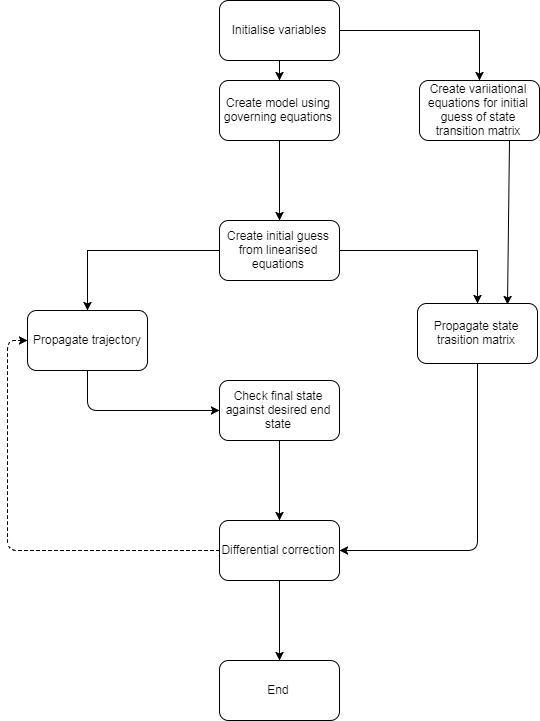
\includegraphics[height = .4\textheight]{figures/softwareFlow}
\caption{Software system architecture for the construction of a periodic orbit about a Lagrangian point.}
\label{f:periodicsoftwareflow}
\end{figure}


Figure \ref{f:periodicsoftwareflow} represents the software runtimes necessary to generate a periodic orbit in the three-body problem. For the remainder of this section, the syntax for the implementation of this computation will be MATLAB-specific, although the heuristics of the work is easily translated into any other computation languages, such as Fortran or Python. 


We first begin by creating the model of the governing equations of motion for the three-body problem. For this case, we restrict the problem to planar motion. Using the governing equations defined in \ref{eq:governingequations},and neglecting the out-of-plane terms, the following parameters are set:

\begin{equation}
	x = 
	\begin{bmatrix}
		x\\
		y\\
		\dot{x}\\
		\dot{y}\\
	\end{bmatrix}
	\dot{x} = 
	\begin{bmatrix}
		\dot{x}\\
		\dot{y}\\
		\dot{v_x}\\
		\dot{v_y}\\
	\end{bmatrix}
\end{equation}

with each initialised through use of a MATLAB vector array, and accessible through the respective array index. $v_x$ and $v_y$ are made available through the governing equations of motion, whilst all other terms are updated by the numerical integration routine.

We now go on to create the variational equations for use in the orbit creation; noting that we are limiting this case to a planar orbit, some modifications of the Jacobian matrix \footnote{Another term for $A(t)$} are required. Recalling equation \ref{eq:jacobianequation}, and neglecting the $U_{xz},~U_{zx},~U_{yz},~U_{zy}$ terms, and reducing $I_3$ to $I_2$ whilst reducing $\Omega$ to be 2x2, yields:

\begin{equation}
	A(t) =
	\begin{bmatrix}
		0 & I_2 \\
		U_{\textnormal{restricted}} & 2\Omega_{\textnormal{restricted}} \\
	\end{bmatrix}
\end{equation}

which we may represent into a model in MATLAB by determining the three double-partial derivatives of the potential function $U(x, y)$ to be 

\begin{equation}
	U_{xx} = -1+\frac{m_1}{r_{13}^{3/2}} \left( 1 - \frac{3(x+m_2)^2}{r_{13}} \right) + \frac{m_2}{r_{23}^{3/2}}\left(1 - \frac{3(x-m_1)^2}{r_{23}}\right)
\end{equation}

\begin{equation}
	U_{yy} = -1 + \frac{m_1}{r_{13}^{3/2}} \left(1-\frac{3y^2}{r_{13}}\right) + \frac{m_2}{r_{23}^{3/2}} \left(1-\frac{3y^2}{4_{23}} \right)
\end{equation}

\begin{equation}
	U_{xy} = -\frac{m_1(3y(x+m_2))}{r_{13}^{5/2}} - \frac{m_2(3y(x-m_1))}{r_{13}^{5/2}}
\end{equation}

Moving on to creating the initial guess from the linearised equations, we refer to \citep{Richardson1980}. Taking the linearised equations of motion about the Lagrange points reference in Equation \ref{eq:linearisedequations}:

\begin{equation}
	\dot{\dot{x}} - 2\dot{y} - (1+2c_2)x = 0
\end{equation}

\begin{equation}
	\dot{\dot{y}} + 2\dot{x} + (c_2+1)y = 0
\end{equation}

\begin{equation}
	\dot{\dot{z}} + \lambda ^2 z = 0
\end{equation}

we obtain a solution in terms of $k$, $c_2$ and $\lambda$, referenced in \ref{eq:amplitudeequations}. Using these as initial solutions, with $\lambda$ as the center eigenvalue, yields:

\begin{equation}
	x = \textnormal{Earth-Sun}~L_i~\textnormal{distance} - A_x
\end{equation}

\noindent where $k$ is equal to:

\begin{equation}
	\frac{1}{2\lambda} \left( \lambda^2 + 1 + 2c_2 \right)
\end{equation}

\noindent and $c_2$ is equal to:

\begin{equation}
	c_2 = \frac{1}{\gamma^3} \left( \mu + \frac{\left( 1 - \mu \right)\gamma ^3}{\left( 1 - \gamma \right)^3} \right)
\end{equation}


%\begin{equation}
%	\frac{1}{\gamma^3} \left( \mu +\frac{\left(1-\mu\right)\gamma^3}{\left(1-\gamma\right)^3}
%:w
%\end{equation}

\noindent with $v_y$ equal to:

\begin{equation}
	v_y = \frac{\textnormal{d}}{\textnormal{d}t} \left(kA_x\sin{\lambda s + \psi}\right) = kA_x\lambda
\end{equation}


\begin{figure}
\centering
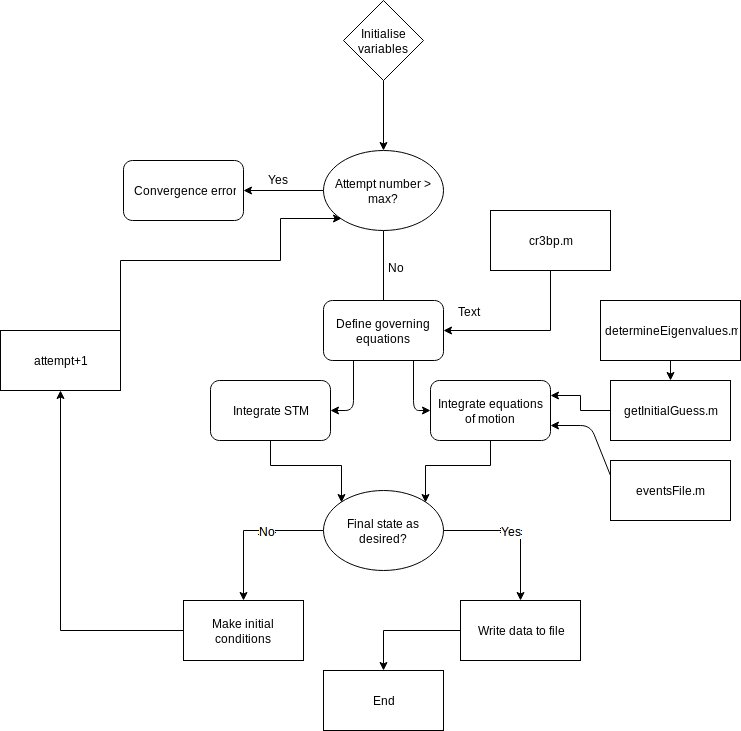
\includegraphics[height=.4\textheight]{figures/differentialCorrectorFlow}
\caption{Differential correction software flow diagram}
\label{f:differentialcorrectorflow}
\end{figure}